\documentclass[9pt]{IEEEtran}

\usepackage[english]{babel}
\usepackage{graphicx}
\usepackage{epstopdf}
\usepackage{fancyhdr}
\usepackage{amsmath}
\usepackage{amsthm}
\usepackage{amssymb}
\usepackage{url}
\usepackage{array}
\usepackage{textcomp}
\usepackage{listings}
\usepackage{hyperref}
\usepackage{xcolor}
\usepackage{colortbl}
\usepackage{float}
\usepackage{gensymb}
\usepackage{longtable}
\usepackage{supertabular}
\usepackage{multicol}
\usepackage{tabu}


\usepackage[utf8x]{inputenc}

\usepackage[T1]{fontenc}
\usepackage{lmodern}
\input{glyphtounicode}
\pdfgentounicode=1

\graphicspath{{./figures/}}
\DeclareGraphicsExtensions{.pdf,.png,.jpg,.eps}

% correct bad hyphenation here
\hyphenation{op-tical net-works semi-conduc-tor trig-gs}

% ============================================================================================

\title{\vspace{0ex}
Web crawler}

\author{Timotej Kovač\vspace{-4.0ex}}

% ============================================================================================

\begin{document}

\maketitle

\section{Introduction}

In this paper we present the structure, challenges and results of a web crawler implementation in Java.
It was used to crawl the *.gov.si websites and produced some interesting results.

\section{Web crawler}

\subsection{Implementation}

For the implementation of the web crawler we used Java and the following support libraries:
\begin{itemize}
\item{Jauntium (which uses Jaunt and Selenium libraries) in order to retrieve web pages and process them using a browser driver and so can also process JavaScript code,}
\item{Robots which is used in order to process the robots.txt files for the domains that will be crawled, }
\item{PostgreSQL which is used to connect and modify the postgres database.}
\end{itemize}

Some other libraries have also been included mostly because the above mentioned ones depend on them.

The frontier is a list that consists of URLs that have yet to be visited.
The initial frontier consists of the starting URLs (see section Constants and issues).
It mainly behaves as a FIFO queue.
But because of the delay limitations that the crawler must obey the process of removing an URL starts as FIFO but skips every record that is not permitted to be visited at this time.

The crawling process begins with the fetch of the robots.txt file for the starting domains. 
Then it initializes multiple workers on seperate threads which then start the process of crawling.
First they gain access to a locked frontier from where they take an available url that has not yet been processed.
Then they update the next permitted window when the domain can be accessed again and proceed with the link processing.

First the program tries to send a HEAD request to get the content type of the target URL.
Because this part of the code offers a much more low level response then when using Jauntium the following redirects must be followed which happens in recursion.
Every URL is here also checked if it has been already crawled and if so the algorithm ends.
If not the data type is extracted from the head of HEAD request or the extension of the URL itself.

The next step is left to the Jauntium to visit the website and it to finish rendering the web page.
The permitted time for this to happen is set to 3000 ms. 

After that the text content of the website is processed so that all of the white space characters are removed. 
If this content matches any other web site in the database the algorithm ends.
If not the websites record in the database is updated with the retrieved information.

The next step are the links and images extraction.
Links are extracted from the website and are added to the frontier if multiple conditions are met.
Some of these are that the URL is a valid URL and not a JavaScript code or anything else, that we haven't visited it yet, that we can visit it based on the robots.txt permissions and so on.
Images are extracted as well and only their source address is added to the database.

After that all of the links that have been extracted are added to the database as well and the crawler thread starts the process again for the next link that is available in the frontier.

\subsection{Parameters and issues}

The crawler implementation does not require any parameters to be set to be able to perform web crawling on the gov.si domains.
There are constants though that can be changed if the user want's to alter the programs result.
These are:
\begin{itemize}
\item{URL\_* strings that define the starting domains that the crawler should start with. Default ones are the gov.si ones.}
\item{THREAD\_COUNT that specifies the number of threads the program will use. It makes sense that this number is at least the same as the number of unique domain names a program will be crawling.}
\item{DELAY specifies the default delay which is used if there isn't a robots.txt file delay specified for that website.}
\item{MAX\_LINKS is used to tell the program when it should stop crawling.}
\item{USER\_AGENT specifies the name of the crawler that will be seen to website servers.}
\end{itemize}

During the implementation of this solution many problems appeared.
It took us a lot of time to make this solution robust to various problems that the crawler might encounter while visiting web sites.

One of the major ones was the retrieval of robots.txt file with robots library. 
Though simple library the URL argument that it requires must be exact.
It does not support any redirects and gov.si websites sometimes start with 'www' and sometimes they don't. 
Also it is necessary to use the whole URL with 'https' at the start as otherwise you won't even get an error but simply an empty file.

The next major thing was the inconsistency of web pages responses to HEAD requests, GET requests, filled out content type (and other) fields, masking of binary data in URLs that don't end with any extension, requests for certificates and redirects to completely different pages which started in URLs with their domain.
This caused most of the effort being spent on implementing a robust way of handling all of the exceptions which appeared. 
Sometimes the website would be fetched but the response would be null.
Other times just getting the list of the available attributes of an HTML element would cause an exception which shouldn't happen.

Regardless the whole implementation has kept a great design even though multiple exceptions had to be made in order not to crash the crawler.

\subsection{Data analysis}

As the result of this crawler working on 6 threads it has taken him 13 hours and 13 minutes to crawl thought 50.000 websites and retrieve their content.
It has crawled though 150 unique gov.si domains and gathered the following amount of content and information:

\begin{table}[ht]{}
\begin{tabu} to 1.0\columnwidth { | X[l] | X[l] | }
\hline
metric & number of webpages  \\
\hline
sites & 150 \\
\hline
pages & 50.002 \\
\hline
binary pages & 284 \\
\hline
...PPTX & 29 \\
\hline
...DOCX & 5 \\
\hline
...PDF & 204 \\
\hline
...DOC & 10 \\
\hline
...PPT & 36 \\
\hline
duplicate pages & 10.110 \\
\hline
\end{tabu}
\caption{Measures comparing unfiltered and filtered detections}
\label{tab2}
\end{table}

As it can be seen from table ~\ref{tab2} 

\subsection{Visualization}

The figure ~\ref{fig1} shows the connections between specific websites and their domains.
Each domain has it's own color and there are four of them.
 
\begin{figure}[h]
    \centering
    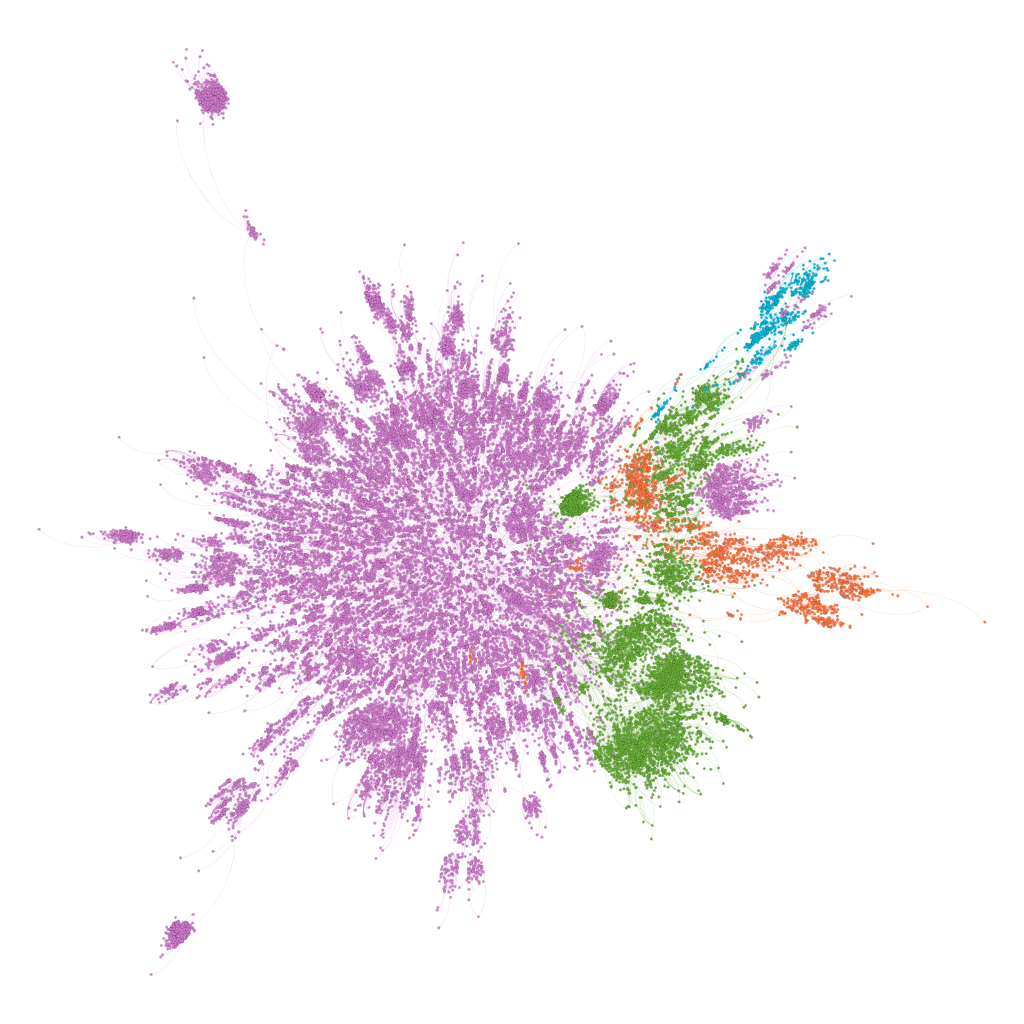
\includegraphics[width=1\columnwidth]{data.png}
    \caption{Graph of links between the pages, where the color represents the domain. Purple is gov.si, green is podatki.gov.si, light blue is gisportal.gov.si, black is evem.gov.si and orange is eugo.gov.si.}
    \label{fig:office}
\end{figure}

\section{Conclusion}

The web crawler implementation was successful in obtaining the content of many of the gov.si websites.
It showed the robustness of it's implementation as the targeted websites had problems and inconsistencies.
It can be used as a general crawler although it is possible that it would require some more work to handle the possible exceptions that it hasn't encounter yet.

\bibliographystyle{IEEEtran}
%\bibliography{bibliography}

\end{document}
